\cleardoublepage % memastikan bab baru dimulai di halaman ganjil (kanan)
\chapter{STUDI LITERATUR}
\label{chap:studi-literatur}
\section{Sistem Tiket Elektronik (\textit{E-Ticket})}
\label{sec:eticket}

Perkembangan teknologi informasi telah mengubah paradigma layanan di berbagai sektor industri, termasuk dalam manajemen akses dan reservasi melalui sistem tiket elektronik atau \textit{e-ticket}. Subbab ini membahas definisi, evolusi, serta karakteristik fundamental dari sistem \textit{e-ticket} yang kini bertransisi menjadi instrumen digital berbasis data.

\subsection{Definisi dan Konsep Dasar}
Menurut Kamus Besar Bahasa Indonesia (KBBI), tiket atau karcis adalah surat kecil (carik kertas khusus) sebagai tanda telah membayar ongkos dan sebagainya (untuk naik bus, menonton bioskop, dan sebagainya). Tiket merupakan dokumen yang berfungsi sebagai bukti hak akses atau tanda pembayaran yang sah untuk menggunakan suatu layanan. Seiring dengan perkembangan teknologi, terjadi transformasi bentuk tiket konvensional yang berbasis kertas menjadi wujud digital yang tersimpan dalam basis data komputer, yang dikenal sebagai \textit{electronic ticket} (\textit{e-ticket}).

Secara konseptual, \textit{e-ticket} bukan sekadar penggantian media kertas, melainkan sebuah kontrak digital yang merepresentasikan hak kepemilikan atas suatu layanan atau produk. Informasi yang sebelumnya tercetak di atas kertas fisik—seperti detail acara, nomor kursi, dan identitas pemegang—kini dikodekan menjadi data digital yang dihubungkan dengan basis data di server pusat. Hal ini memungkinkan proses validasi dilakukan secara instan melalui pencocokan data digital, bukan sekadar pemeriksaan visual fisik kertas.

\subsection{Evolusi dan Transformasi Digital}
Pergeseran menuju \textit{e-ticket} merupakan bagian dari proses inovasi layanan yang lebih luas. Dalam konteks transportasi publik, \textcite{lubeck2012electronic} menjelaskan bahwa tiket elektronik dikembangkan sebagai evolusi dari sistem kartu pita magnetik dan tiket kertas konvensional. Pengembangan ini didorong oleh kekhawatiran akan inefisiensi dalam manajemen informasi dan lemahnya kontrol operasi pada sistem terdahulu.

Pada fase awal, sistem konvensional seringkali terkendala oleh keterbatasan dalam pelacakan data dan audit transaksi. Adopsi sistem teknis terkomputerisasi kemudian muncul sebagai solusi untuk meningkatkan efisiensi dan efektivitas operasional. Menurut \textcite{lubeck2012electronic}, implementasi sistem tiket elektronik merupakan bentuk inovasi proses yang merampingkan dan mengkualifikasi operasional dengan mengurangi proses manual sehingga meningkatkan kualitas layanan secara keseluruhan. Transformasi ini mengubah cara pengelolaan informasi karena sistem kini mampu meregistrasi pengguna, mengontrol alokasi tiket, dan menerbitkan laporan manajemen yang akurat untuk pemantauan data secara terpusat.

\subsection{Keunggulan dan Tantangan Operasional}
Adopsi luas sistem \textit{e-ticket} didorong oleh berbagai keunggulan signifikan dibandingkan sistem konvensional. \textcite{chen2007passenger} menyoroti bahwa motivasi utama peralihan ke \textit{e-ticketing} adalah penghematan biaya distribusi tiket dan pemangkasan biaya penanganan (\textit{handling overheads}). Sistem ini memungkinkan eliminasi tiket kertas yang berdampak langsung pada pengurangan biaya tenaga kerja, pencetakan, pengiriman, dan akuntansi. Bagi pengguna, manfaat utamanya adalah kenyamanan akibat sifat tiket yang \textit{paperless}, yang secara spesifik menghilangkan risiko kehilangan fisik tiket sebelum acara atau perjalanan berlangsung.

Di sisi lain, \textcite{lubeck2012electronic} menekankan bahwa keuntungan krusial dari \textit{e-ticket} terletak pada peningkatan manajemen informasi dan kontrol operasional. Sistem ini efektif membatasi perdagangan tiket ilegal (\textit{illegal trade}) yang sebelumnya marak terjadi pada tiket fisik, serta mempersulit penyalahgunaan manfaat tiket khusus (seperti tiket pelajar atau tarif subsidi) karena identitas tiket kini bersifat personal dan terikat pada akun pengguna. Selain itu, sistem elektronik juga meningkatkan keamanan fisik dengan meminimalkan peredaran uang tunai (\textit{cashless transaction}) di lokasi layanan.

Namun, di balik efisiensi tersebut, sistem \textit{e-ticket} berbasis peladen terpusat melahirkan tantangan operasional baru [Perlu Sitasi: Jurnal/makalah terkait tantangan ketersediaan jaringan pada infrastruktur \textit{smart ticketing}]. Ketergantungan yang mutlak pada basis data pusat mewajibkan tersedianya konektivitas jaringan internet yang stabil di setiap titik pemeriksaan (\textit{gate}). Ketika terjadi kegagalan jaringan atau lonjakan antrean yang memicu kejenuhan trafik (\textit{network congestion}), proses validasi di lapangan akan terhenti total. Kondisi ini menuntut adanya perancangan mekanisme validasi mandiri (\textit{offline validation}) yang mampu memverifikasi keaslian tiket secara lokal tanpa mengorbankan integritas keamanan data.

\section{Teknologi \textit{Quick Response} Kode (QR)}
\label{sec:qrcode}

\subsection{Sejarah dan Prinsip Kerja}
\textit{Quick Response Code} (Kode QR) adalah jenis kode batang matriks dua dimensi yang dikembangkan oleh Denso Wave pada tahun 1994. Awalnya ditujukan untuk pelacakan inventaris suku cadang industri otomotif, teknologi ini kini telah diadopsi secara masif di berbagai sektor mulai dari pemasaran digital hingga manajemen kontrol akses \cite{tiwari2016introduction, shin2012psychology}. \textcite{shin2012psychology} mendefinisikan kode QR sebagai pola persegi yang terdiri dari modul hitam dengan latar belakang putih yang dirancang untuk didekodekan dengan kecepatan tinggi menggunakan perangkat pemindai optik atau kamera ponsel pintar.

Berbeda dengan kode batang (\textit{barcode}) satu dimensi yang hanya menyimpan data secara horizontal, kode QR mengodekan informasi dalam dua dimensi, yaitu vertikal dan horizontal. Struktur dua dimensi ini memungkinkan kode QR memiliki densitas informasi yang jauh lebih tinggi dan kapasitas penyimpanan yang lebih besar dalam ruang fisik yang lebih kecil dibandingkan pendahulunya \cite{alsuhibany2025innovative}. Kapasitas ini memungkinkan penyimpanan berbagai mode data, termasuk numerik, alfanumerik, biner (byte), hingga karakter Kanji \cite{tiwari2016introduction}, yang menjadikannya medium ideal untuk mentransmisikan muatan data (\textit{payload}) tiket elektronik yang kompleks.

\subsection{Struktur Kode QR}
Kemampuan kode QR untuk dibaca dengan kecepatan tinggi dan akurasi tinggi (\textit{high-speed reading}) didukung oleh tata letak strukturnya yang terstandarisasi. Berdasarkan spesifikasi teknis yang dijelaskan oleh \textcite{tiwari2016introduction}, setiap simbol kode QR dibangun dari modul-modul persegi yang disusun dalam \textit{array} persegi reguler. Struktur ini terdiri dari dua bagian utama, yaitu pola fungsi (\textit{function patterns}) dan wilayah pengodean (\textit{encoding region}), yang dikelilingi oleh batas zona tenang (\textit{quiet zone}) di keempat sisinya.

Wilayah pengodean (\textit{encoding region}) berisi modul-modul data yang merepresentasikan informasi versi, informasi format, data muatan (\textit{payload}), dan \textit{codeword} koreksi kesalahan. Sementara itu, pola fungsi adalah bentuk-bentuk spesifik yang ditempatkan di area tertentu untuk memastikan pemindai dapat mengidentifikasi, mengukur ukuran modul, dan mengorientasikan kode dengan benar. Komponen visual utama kode QR diilustrasikan pada Gambar \ref{fig:struktur_qrcode}, dengan rincian elemen dijelaskan sebagai berikut:

\begin{figure}[h]
    \centering
    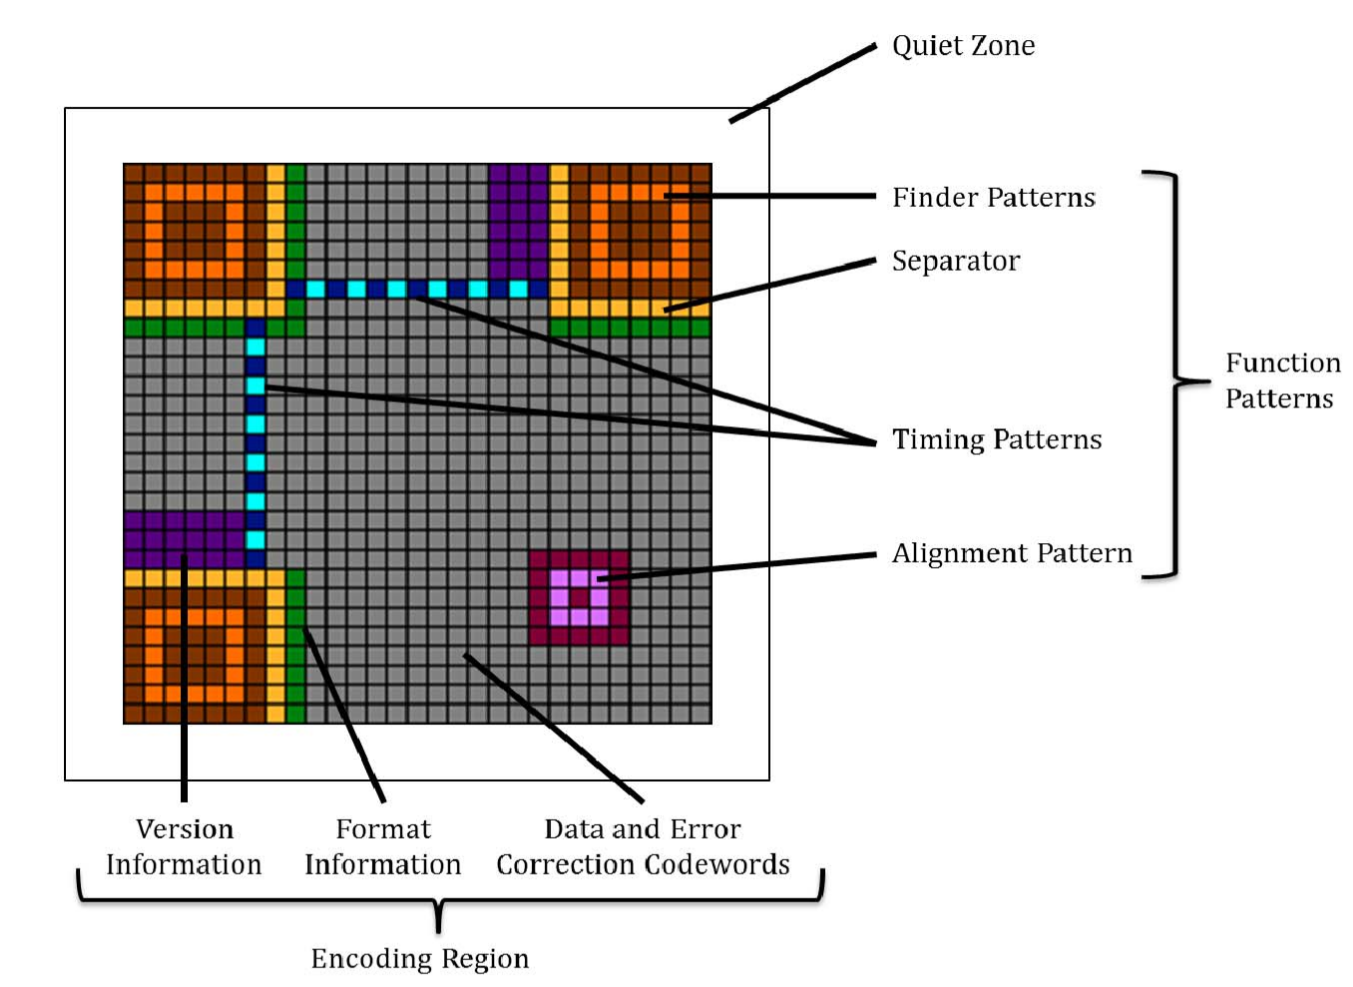
\includegraphics[width=0.8\textwidth]{images/struktur_qrcode.png} 
    \caption{Struktur Kode QR \cite{tiwari2016introduction}}
    \label{fig:struktur_qrcode}
\end{figure}

\begin{enumerate}[a)]
    \item \textbf{\textit{Finder Pattern}: }
    Tiga struktur kotak konsentris yang terletak di sudut kiri atas, kanan atas, dan kiri bawah simbol. Pola ini memungkinkan pemindai mendeteksi posisi dan sudut rotasi kode dari segala arah (360 derajat), sehingga pemindaian dapat dilakukan secara serbaguna (\textit{omni-directional}).
    
    \item \textbf{\textit{Separators}: }
    Area selebar satu modul berwarna putih yang membatasi setiap \textit{finder pattern} dari wilayah pengodean (\textit{encoding region}) untuk mencegah interferensi deteksi pola.

    \item \textbf{\textit{Alignment Pattern}: }
    Pola kotak kecil di kuadran kanan bawah yang berfungsi mengoreksi distorsi geometris jika kode dipindai pada permukaan melengkung atau sudut pandang miring.
    
    \item \textbf{\textit{Timing Pattern}: }
    Garis modul hitam-putih berselang-seling yang menghubungkan pola pencari guna menentukan koordinat modul kisi dan tingkat densitas simbol.
    
    \item \textbf{\textit{Quiet Zone}: }
    Area margin kosong di sekeliling simbol (minimal selebar empat modul) yang memisahkan kode dari noise visual atau elemen grafis di latar belakang.
\end{enumerate}

\subsection{Koreksi Kesalahan (\textit{Error Correction})}
Salah satu keunggulan teknis kode QR yang paling krusial untuk implementasi \textit{e-ticket} adalah kemampuan koreksi kesalahan berbasis algoritma Reed-Solomon. Fitur ini memungkinkan data tetap dapat didekodekan secara utuh meskipun sebagian area simbol mengalami kerusakan fisik, tergores, atau kotor \cite{tiwari2016introduction}. Tingkat koreksi kesalahan dibagi menjadi empat tingkatan standar sebagaimana ditampilkan pada Tabel \ref{tab:error_correction}.

\begin{table}[htbp]
    \centering
    \caption{Tingkat Koreksi Kesalahan (\textit{Error Correction Level}) pada kode QR \cite{tiwari2016introduction}}
    \label{tab:error_correction}
    % Menggunakan tabularx dengan garis vertikal (|) untuk membuat grid
    \begin{tabularx}{\textwidth}{| c | >{\raggedright\arraybackslash}X | c |}
        \hline
        \textbf{Level} & \textbf{Keterangan} & \textbf{Kemampuan Pemulihan Data} \\
        \hline
        L & \textit{Low} (Rendah) & $\approx$ 7\% \\
        \hline
        M & \textit{Medium} (Menengah) & $\approx$ 15\% \\
        \hline
        Q & \textit{Quartile} (Tinggi) & $\approx$ 25\% \\
        \hline
        H & \textit{High} (Sangat Tinggi) & $\approx$ 30\% \\
        \hline
    \end{tabularx}
\end{table}

Pemilihan level koreksi kesalahan ini menghadirkan pertukaran (\textit{trade-off}) antara ketahanan fisik kode dan kapasitas muatan data: semakin tinggi level koreksi yang dipilih, semakin banyak modul yang dialokasikan untuk \textit{codeword} redundansi, sehingga mengurangi kapasitas data efektif. Level M (15\%) atau Level Q (25\%) umumnya direkomendasikan untuk tiket elektronik seluler guna mengantisipasi goresan layar atau pantulan cahaya saat pemindaian berlangsung \cite{tiwari2016introduction}.

\subsection{Kode QR Statis vs. Dinamis}
Dalam implementasi sistem informasi tiket, kode QR diklasifikasikan berdasarkan sifat data dan perilakunya:

\begin{enumerate}[a)]
    \item \textbf{Kode QR Statis:} Muatan data dienkodekan secara langsung dan permanen ke dalam pola matriks citra. Karakteristik dasarnya adalah informasi bersifat tetap (\textit{fixed information}) dan tidak dapat diubah setelah dibangkitkan. \textcite{yanuarafi2023perbandingan} mencatat bahwa tipe ini memiliki kerentanan keamanan tinggi karena pola visualnya yang permanen memungkinkan pelaku kejahatan menduplikasi dan menyebarkannya secara massal.
    
    \item \textbf{Kode QR Dinamis (Umum):} Dalam praktik industri umum, kode QR dinamis memuat tautan pendek (\textit{short URL}) yang mengarahkan peramban pengguna ke peladen web. Pola visual QR tetap sama, namun konten tujuan di peladen dapat diperbarui. Meskipun fleksibel, model ini masih rentan terhadap penggandaan citra jika tautan di dalamnya tidak dilengkapi lapisan autentikasi sesi yang ketat.

    \item \textbf{Kode QR Dinamis Berbasis Waktu (Konteks Tugas Akhir):} Berbeda dengan pendekatan tautan statis di atas, penelitian ini mengadopsi mekanisme di mana muatan data (\textit{payload}) internal kode QR dihitung ulang dan diperbarui secara periodik menggunakan algoritma berbasis waktu (\textit{Time-based One-Time Password} / TOTP). Pola visual matriks berubah secara berkala dalam interval detik. \textcite{sung2015security} menegaskan pentingnya mekanisme kedaluwarsa (\textit{expiration}) otomatis ini untuk membatasi masa berlaku tampilan tiket, sehingga salinan hasil tangkapan layar (\textit{screenshot}) akan segera kedaluwarsa dan ditolak oleh sistem pemindai.
\end{enumerate}

\section{Ancaman dan Kerentanan pada Sistem \textit{E-Ticket}}
\label{sec:keamanan_eticket}

Dalam konteks rekayasa keamanan sistem informasi, penting untuk membedakan secara tegas antara ancaman (\textit{threat}) dan vektor serangan (\textit{attack vector}). Ancaman merujuk pada potensi kejadian merugikan yang mengancam integritas operasional, kerugian finansial, atau reputasi penyelenggara acara. Sementara itu, vektor serangan adalah teknik teknis spesifik yang dieksploitasi oleh penyerang untuk merealisasikan ancaman tersebut pada sistem tiket statis.

\subsection{Identifikasi Ancaman (\textit{Threat Landscape})}
Berdasarkan studi empiris dan literatur terkini, lanskap ancaman pada ekosistem pertiketan digital dikelompokkan menjadi empat isu utama:

\begin{enumerate}[a)]
    \item \textbf{Praktik Percaloan (\textit{Scalping}): }
    Calo menurut Kamus Besar Bahasa Indonesia (KBBI) didefinisikan sebagai perantara yang memberikan jasanya berdasarkan upah. Dalam konteks pertiketan, percaloan merupakan ancaman distorsi pasar di mana pelaku memborong tiket secara terorganisasi lalu menjualnya kembali dengan harga yang melonjak berkali-kali lipat dari harga resmi \cite{Pamela2023}. Praktik ini mengeksploitasi kelonggaran transfer tiket digital statis dan sangat merugikan hak konsumen.
        
    \item \textbf{Penipuan Tiket (\textit{Fraud}): }
    Ancaman kejahatan berupa penjualan tiket palsu atau penjualan satu salinan tiket asli yang sama kepada banyak korban secara berulang. Investigasi \textcite{diveranta2025jejak} menunjukkan kerugian publik mencapai miliaran rupiah akibat peredaran tiket duplikat di pasar sekunder ilegal.

    \item \textbf{Infiltrasi Akses Ilegal: }
    Ancaman operasional di mana penonton tanpa hak akses sah berhasil memasuki area acara. Kondisi ini memicu ketidaknyamanan fatal bagi pemegang tiket asli yang hak kursinya terampas, serta melipatgandakan risiko keamanan di dalam stadion atau gedung pertunjukan \cite{Kurniawan2024}.

    \item \textbf{Kegagalan Titik Tunggal (\textit{Single Point of Failure / SPoF}): }
    Ancaman sistemik yang muncul akibat ketergantungan mutlak pada konektivitas peladen pusat. \textcite{lever2013single} mendefinisikan SPoF sebagai kegagalan pada satu komponen kritis yang meruntuhkan fungsionalitas seluruh sistem terintegrasi. \textcite{jafarnejad2017load} menegaskan bahwa arsitektur terpusat (\textit{centralized}) memiliki titik kritis saat terjadi lonjakan trafik; jika peladen mengalami kelebihan beban (\textit{overload}) atau koneksi terputus, seluruh gerbang pemindai di lokasi acara akan mengalami kelumpuhan operasional total.
\end{enumerate}

\subsection{Analisis Vektor Serangan Teknis (\textit{Attack Vectors})}
Untuk mewujudkan ancaman di atas, pelaku kejahatan memanfaatkan celah arsitektur kode QR statis melalui empat vektor serangan utama:

\begin{enumerate}[a)]
    \item \textbf{Serangan Penggandaan (\textit{Cloning Attack}): }
    Pelaku mengeksploitasi sifat visual kode QR statis dengan menyalinnya melalui fitur tangkapan layar (\textit{screen capture}) pada ponsel pintar \cite{sung2015security}. Karena arsitektur statis tidak dapat membedakan antara tampilan langsung aplikasi resmi dengan gambar salinan di galeri foto, tiket duplikat tersebut dapat diperjualbelikan kepada korban tanpa disadari oleh sistem.
    
    \item \textbf{Serangan Putar Ulang (\textit{Replay Attack}): }
    Serangan ini mengeksploitasi data tiket sah yang ditangkap lalu dikirimkan ulang (\textit{replayed}) pada alat pemindai. Tanpa adanya pembatasan jendela waktu yang ketat (\textit{time-bound}) dan pengikatan spasial (\textit{location-bound}), tiket yang sama dapat digunakan berulang kali atau dipindai secara simultan pada dua pintu masuk yang berbeda dalam kondisi luring (\textit{Multi-Gate Offline Replay}) [Perlu Sitasi: Jurnal/makalah keamanan sistem mengenai celah replikasi/penyusupan simultan pada token berbasis waktu pada arsitektur terdistribusi tanpa koneksi \textit{real-time}].
    
    \item \textbf{Eksfiltrasi Data dan Kunci (\textit{Data \& Key Exfiltration}): }
    Serangan yang menargetkan penyimpanan lokal (\textit{local storage}) perangkat pengguna melalui malware atau celah sistem operasi \cite{sung2015security}. Jika data identitas pribadi (\textit{Personally Identifiable Information} / PII) atau kunci pembangkit token disimpan secara terbuka (\textit{plaintext}), data tersebut rentan dicuri untuk merekonstruksi tiket palsu. Hal ini menuntut penerapan prinsip \textit{Data Minimization} pada muatan data tiket.
    
    \item \textbf{Rekayasa Balik (\textit{Reverse Engineering}): }
    Penyerang berupaya membongkar kode biner aplikasi pengguna atau alat pemindai untuk menemukan kunci kriptografi statis (\textit{hardcoded master secret}). Jika kunci rahasia berhasil diekstrak dari perangkat pemindai, penyerang dapat menerbitkan tiket palsu yang secara matematis valid di hadapan sistem luring. Ancaman ini menegaskan perlunya skema kriptografi asimetris di mana pemindai hanya memegang kunci publik verifikasi.
\end{enumerate}

\section{Landasan Teori Kriptografi untuk Solusi}
\label{sec:kriptografi}

Solusi keamanan yang diusulkan dalam penelitian ini, yaitu \textit{Dynamic Secure QR Code}, dibangun di atas fondasi algoritma kriptografi modern. Subbab ini menguraikan konsep teoretis dari teknologi kriptografi yang digunakan, membedah operasi matematis di balik kriptografi asimetris, pembentukan tanda tangan digital berbasis kurva eliptik, fungsi \textit{Hash-based Message Authentication Code} (HMAC) beserta derivasi kunci, serta mekanisme pemangkasan dinamis (\textit{dynamic truncation}) pada algoritma \textit{Time-based One-Time Password} (TOTP).

\subsection{Kriptografi Asimetris dan Kurva Eliptik (\textit{Elliptic Curve Cryptography})}
Kriptografi asimetris, atau sering disebut kriptografi kunci publik, merupakan konsep fundamental dalam keamanan informasi modern yang diperkenalkan untuk mengatasi kelemahan distribusi kunci pada kriptografi simetris [Perlu Sitasi: Buku David Wong (Real-World Cryptography, Bab 1) / Stallings]. Skema ini menggunakan sepasang kunci berbeda yang saling berkaitan secara matematis, yaitu kunci publik (\textit{public key}) dan kunci privat (\textit{private key}).

Skema kriptografi asimetris beroperasi melalui fungsi satu arah dengan jebakan (\textit{trapdoor one-way function}). Secara teoretis, skema ini dapat digunakan untuk tujuan kerahasiaan (\textit{confidentiality}) sebagaimana diilustrasikan pada Gambar \ref{fig:enkripsi_publik}, di mana data dienkripsi dengan kunci publik penerima dan hanya dapat didekripsi oleh kunci privat pemilik. Namun, dalam konteks arsitektur \textit{e-ticket} penelitian ini, fungsi kriptografi asimetris difokuskan pada aspek autentikasi dan integritas data (Gambar \ref{fig:enkripsi_privat}), di mana kunci privat digunakan oleh peladen pusat untuk menandatangani data tiket, sedangkan kunci publik didistribusikan ke perangkat pemindai untuk memverifikasi keabsahan tiket secara mandiri dalam mode \textit{offline} [Perlu Sitasi: Buku David Wong, Bab 1 Bagian 1.4].

\begin{figure}[t]
    \centering
    % --- Sub-gambar A (Posisi Atas) ---
    \begin{subfigure}[b]{\textwidth} 
        \centering
        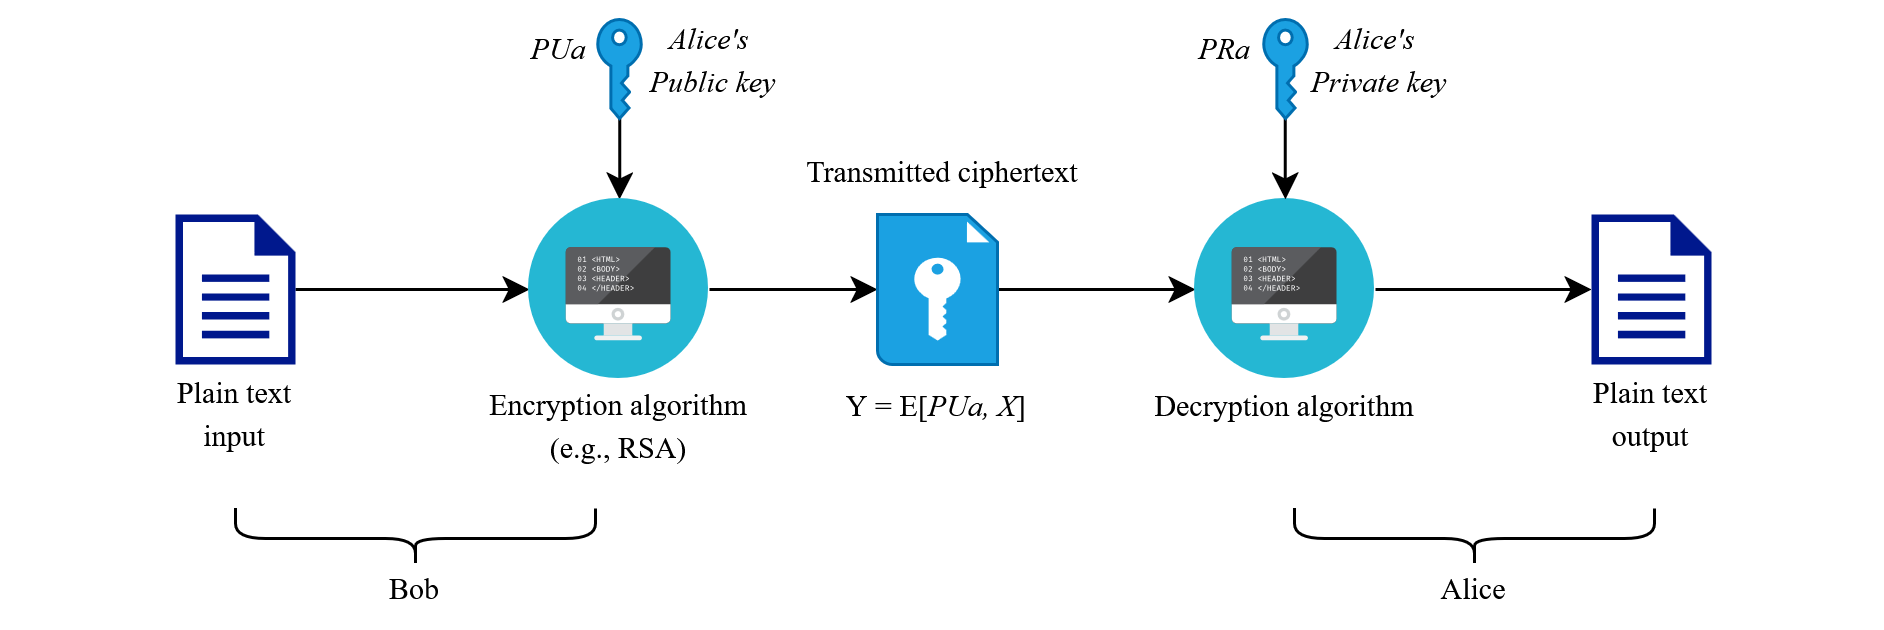
\includegraphics[width=\textwidth]{images/encrypt_1.png} 
        \caption{Enkripsi Kunci Publik (Kerahasiaan)}
        \label{fig:enkripsi_publik}
    \end{subfigure}
    
    \vspace{1cm} 
    
    % --- Sub-gambar B (Posisi Bawah) ---
    \begin{subfigure}[b]{\textwidth}
        \centering
        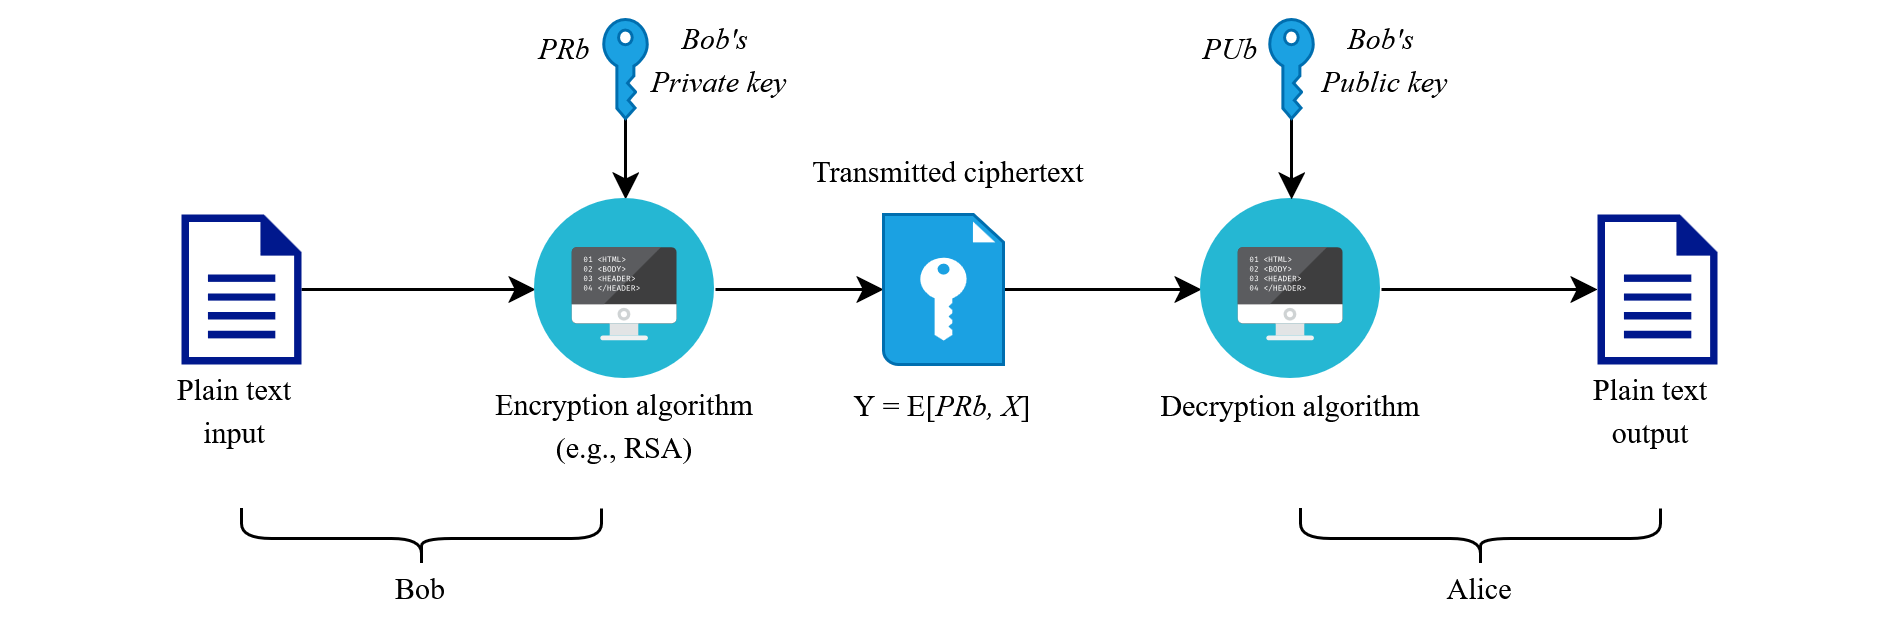
\includegraphics[width=\textwidth]{images/encrypt_2.png}
        \caption{Enkripsi Kunci Privat (Autentikasi)}
        \label{fig:enkripsi_privat}
    \end{subfigure}
    
    \caption{Skema Enkripsi Kunci Publik \cite{stallings2022cryptography}}
    \label{fig:skema_pkc}
\end{figure}

Berbeda dengan algoritma RSA tradisional yang mendasarkan keamanannya pada tingkat kesulitan komputasi faktorisasi bilangan prima besar, penelitian ini mengadopsi \textit{Elliptic Curve Cryptography} (ECC). Keamanan matematis ECC didasarkan pada Masalah Logaritma Diskrit Kurva Eliptik (\textit{Elliptic Curve Discrete Logarithm Problem} / ECDLP) [Perlu Sitasi: Buku David Wong, Bab 5 Bagian 5.3]. Secara matematis, kurva eliptik yang didefinisikan pada lapangan hingga prima $\mathbb{F}_p$ umumnya dinyatakan dalam bentuk persamaan Weierstrass tereduksi:
\begin{equation}
    y^2 \equiv x^3 + ax + b \pmod p
\end{equation}
dengan konstanta $a, b \in \mathbb{F}_p$ yang memenuhi kondisi diskriminan non-singular $4a^3 + 27b^2 \not\equiv 0 \pmod p$.

Dalam domain grup kurva eliptik, operasi penjumlahan titik (\textit{point addition}) dan penggandaan titik (\textit{point doubling}) memungkinkan dilakukannya operasi perkalian skalar:
\begin{equation}
    P = [x]G = \underbrace{G + G + \dots + G}_{x \text{ kali}}
\end{equation}
di mana $G$ adalah titik generator kurva (titik basis dengan orde prima $n$), $x \in [1, n-1]$ adalah bilangan skalar yang bertindak sebagai kunci privat, dan $P$ adalah titik hasil yang bertindak sebagai kunci publik [Perlu Sitasi: Buku David Wong, Bab 5]. Sifat dasar ECDLP menyatakan bahwa dengan mengetahui titik $G$ dan titik hasil $P$, secara komputasi tidak layak (\textit{infeasible}) untuk menemukan kembali nilai skalar privat $x$. 

Karakteristik ini memungkinkan ECC menawarkan kekuatan kriptografi yang setara dengan RSA namun dengan ukuran kunci yang jauh lebih ringkas. Sebagai contoh, kunci ECC dengan panjang 256-bit (seperti pada kurva standar NIST P-256 atau secp256k1) memberikan tingkat keamanan 128-bit yang setara dengan kunci RSA 3072-bit [Perlu Sitasi: Publikasi NIST SP 800-57 atau studi efisiensi kurva eliptik]. Ukuran kunci dan tanda tangan yang sangat ringkas ini menjadi keunggulan utama untuk efisiensi muatan data (\textit{payload}) kode QR pada sistem \textit{e-ticket}.

\subsection{Tanda Tangan Digital ECDSA}
Tanda tangan digital merupakan mekanisme kriptografi yang memberikan tiga jaminan keamanan fundamental: autentikasi asal data (\textit{origin authentication}), integritas pesan (\textit{message integrity}), dan nirsangkal (\textit{non-repudiation}) [Perlu Sitasi: Buku David Wong, Bab 7 Bagian 7.1]. Pada penelitian ini, algoritma yang digunakan adalah \textit{Elliptic Curve Digital Signature Algorithm} (ECDSA), yaitu varian standar ANSI X9.62 dan FIPS 186-4 dari algoritma DSA yang diadaptasi pada struktur kurva eliptik.

Proses pembentukan tanda tangan digital ECDSA oleh peladen pusat terhadap muatan data tiket $m$ dieksekusi melalui tahapan matematis berikut:
\begin{enumerate}
    \item Menghitung nilai intisari (\textit{hash digest}) dari pesan $m$ menggunakan fungsi hash kriptografi (misalnya SHA-256), lalu memotong nilai tersebut sesuai panjang bit orde kurva: $e = H(m)$.
    \item Memilih sebuah bilangan acak rahasia sekali pakai (\textit{nonce}) $k$ secara seragam dari interval $[1, n-1]$.
    \item Menghitung titik kurva hasil perkalian skalar: $(x_1, y_1) = [k]G$.
    \item Menghitung komponen tanda tangan pertama ($r$) sebagai koordinat $x_1$ modulo $n$:
    \begin{equation}
        r = x_1 \pmod n
    \end{equation}
    Jika diperoleh $r = 0$, proses diulang dengan memilih nilai $k$ baru.
    \item Menghitung komponen tanda tangan kedua ($s$) menggunakan kunci privat peladen $d_A$:
    \begin{equation}
        s = k^{-1} (e + r \cdot d_A) \pmod n
    \end{equation}
    di mana $k^{-1}$ adalah invers perkalian modular dari $k$ modulo $n$. Jika diperoleh $s = 0$, proses diulang dengan nilai $k$ baru.
\end{enumerate}

Tanda tangan digital yang dihasilkan merupakan pasangan skalar integer $(r, s)$. Pada sisi alat pemindai, proses verifikasi dijalankan secara luring (\textit{offline}) menggunakan kunci publik peladen $Q_A = [d_A]G$ melalui langkah verifikasi persamaan kurva:
\begin{equation}
    w = s^{-1} \pmod n, \quad u_1 = e \cdot w \pmod n, \quad u_2 = r \cdot w \pmod n
\end{equation}
\begin{equation}
    (x_2, y_2) = [u_1]G + [u_2]Q_A
\end{equation}
Tanda tangan dinyatakan sah (\textit{valid}) jika dan hanya jika $x_2 \equiv r \pmod n$. Skema ini memastikan bahwa tiket digital diterbitkan oleh peladen resmi yang sah dan belum mengalami modifikasi data oleh pihak ketiga.

\subsection{HMAC dan Fungsi Derivasi Kunci (\textit{Key Derivation})}
\label{sec:hmac_kdf}
\textit{Hash-based Message Authentication Code} (HMAC) merupakan algoritma autentikasi pesan berbasis kunci simetris yang menggabungkan fungsi hash kriptografis dengan kunci rahasia bersama [Perlu Sitasi: Buku David Wong, Bab 3 Bagian 3.5]. Sesuai dengan spesifikasi IETF RFC 2104, formulasi komputasi internal HMAC didefinisikan sebagai:
\begin{equation}
    HMAC(K, m) = H\Big((K \oplus opad) \parallel H\big((K \oplus ipad) \parallel m\big)\Big)
\end{equation}
di mana:
\begin{itemize}
    \item $K$ adalah kunci rahasia yang telah disesuaikan panjangnya dengan ukuran blok fungsi hash.
    \item $m$ adalah pesan masukan yang akan diautentikasi.
    \item $H$ adalah fungsi hash kriptografis iteratif (seperti SHA-256).
    \item $ipad$ (\textit{inner padding}) adalah konstanta biner berulang \texttt{0x36}.
    \item $opad$ (\textit{outer padding}) adalah konstanta biner berulang \texttt{0x5C}.
    \item Simbol $\oplus$ melambangkan operasi logika \textit{Exclusive OR} (XOR) dan $\parallel$ melambangkan konkatenasi (penggabungan) biner.
\end{itemize}

Selain berfungsi sebagai kode autentikasi pesan, konstruksi HMAC memiliki sifat \textit{pseudorandom function} (PRF) yang terbukti aman terhadap serangan manipulasi ekstensi panjang (\textit{length extension attack}) [Perlu Sitasi: Buku David Wong, Bab 3]. Sifat ini menjadikannya landasan ideal untuk Fungsi Derivasi Kunci (\textit{Key Derivation Function} / KDF), seperti pada standar HKDF (RFC 5869) dan NIST SP 800-108.

Dalam arsitektur penelitian ini, KDF berbasis HMAC dimanfaatkan untuk menurunkan kunci rahasia gerbang (\textit{gate-specific secret}) dan kunci token pengguna dari sebuah kunci induk (\textit{Master Secret}):
\begin{equation}
    K_{derived} = HMAC(K_{master}, Context)
\end{equation}
di mana $Context$ berisi pengidentifikasi unik gerbang atau ID tiket. Mekanisme ini memungkinkan perangkat pemindai merekonstruksi kunci validasi lokal secara dinamis (\textit{stateless validation}) tanpa perlu menyimpan basis data seluruh kunci tiket pengguna, sehingga meminimalkan risiko kebocoran kunci massal pada penyimpanan lokal alat pemindai.

\subsection{Algoritma TOTP dan Mekanisme \textit{Dynamic Truncation}}
Untuk menghasilkan kode QR dinamis yang memiliki jendela kedaluwarsa otomatis terhadap waktu, penelitian ini menerapkan algoritma \textit{Time-based One-Time Password} (TOTP) yang distandardisasi dalam RFC 6238. TOTP merupakan evolusi dari algoritma berbasis kejadian \textit{HMAC-based One-Time Password} (HOTP, RFC 4226) yang menggantikan pencacah sekuensial ($C$) dengan parameter waktu berbasis detik (\textit{Unix epoch}) [Perlu Sitasi: RFC 6238 / RFC 4226].

Perhitungan langkah waktu diskrit ($T$) dirumuskan sebagai:
\begin{equation}
    T = \left\lfloor \frac{CurrentTime - T_0}{X} \right\rfloor
\end{equation}
di mana $CurrentTime$ adalah waktu saat ini dalam detik, $T_0$ adalah waktu awal acuan (lazimnya 0), dan $X$ adalah durasi jendela waktu pembaruan kode (misalnya 30 detik). Nilai integer 64-bit $T$ ini kemudian diproses ke dalam fungsi HMAC bersama kunci rahasia bersama $K$:
\begin{equation}
    HS = HMAC\text{-}SHA\text{-}256(K, T)
\end{equation}

Keluaran $HS$ menghasilkan deret biner sepanjang 32 byte (256 bit). Untuk mengonversi deret hash yang panjang ini menjadi kode numerik 6 digit yang ringkas pada kode QR, algoritma menerapkan proses pemotongan dinamis (\textbf{\textit{Dynamic Truncation}} / DT) sesuai RFC 4226 melalui empat langkah operasional:
\begin{enumerate}
    \item \textbf{Ekstraksi Offset (\textit{Offset Extraction}): } 
    Membaca 4 bit berorde rendah (\textit{low-order bits}) dari byte terakhir deret hash untuk menentukan indeks pergeseran (\textit{offset}):
    \begin{equation}
        Offset = HS[31] \ \& \ \texttt{0x0F}
    \end{equation}
    Operasi ini menghasilkan nilai integer $Offset \in [0, 15]$.
    
    \item \textbf{Ekstraksi 4-Byte (\textit{4-Byte Extraction}): }
    Mengambil irisan biner sepanjang 4 byte (32 bit) dari $HS$ yang dimulai dari indeks $Offset$:
    \begin{equation}
        P = HS[Offset \dots Offset+3]
    \end{equation}
    
    \item \textbf{Operasi Masking Bitwise: }
    Melakukan operasi \texttt{AND} terhadap nilai 32-bit $P$ dengan masker heksadesimal \texttt{0x7FFFFFFF}:
    \begin{equation}
        S_{num} = P \ \& \ \texttt{0x7FFFFFFF}
    \end{equation}
    Langkah ini bertujuan membuang \textit{Most Significant Bit} (MSB) agar hasil integer 31-bit selalu bernilai positif pada komputasi bertanda (\textit{signed arithmetic}).
    
    \item \textbf{Reduksi Modulo (\textit{Modulo Reduction}): }
    Nilai biner $S_{num}$ kemudian dikonversi menjadi digit desimal dengan menerapkan operasi modulo terhadap $10^d$, di mana $d$ adalah jumlah digit token yang diinginkan (untuk $d = 6$ digit):
    \begin{equation}
        TOTP = S_{num} \pmod{10^6}
    \end{equation}
\end{enumerate}

Melalui formulasi matematis di atas, sistem menghasilkan token 6 digit dinamis yang terikat pada jendela waktu tertentu. Kode QR yang dibangkitkan dari token ini akan otomatis kedaluwarsa setelah interval waktu $X$ berakhir, sehingga mematahkan serangan penggandaan tiket via tangkapan layar (\textit{screenshot cloning}) dan serangan putar ulang (\textit{replay attack}).

\section{Teknologi \textit{Bluetooth Low Energy} (BLE) dan Mekanisme \textit{Beacon}}
\label{sec:ble_beacon}

Untuk memastikan bahwa tiket dinamis tidak hanya valid dalam dimensi waktu (melalui TOTP) tetapi juga terikat secara spasial pada lokasi fisik gerbang masuk, penelitian ini mengintegrasikan teknologi \textit{Bluetooth Low Energy} (BLE). Subbab ini menguraikan arsitektur komunikasi BLE, model propagasi sinyal proksimitas, serta formulasi mekanisme pengikatan gerbang (\textit{Gate-Bound}).

\subsection{Arsitektur dan Kanal Transmisi BLE}
\textit{Bluetooth Low Energy} (BLE) merupakan teknologi jaringan area personal nirkabel (\textit{Wireless Personal Area Network} / WPAN) yang distandardisasi oleh Bluetooth Special Interest Group (SIG) untuk aplikasi dengan konsumsi daya dan latensi yang sangat rendah [Perlu Sitasi: Spesifikasi Inti Bluetooth SIG / Buku Pengantar BLE]. Berbeda dengan Bluetooth Klasik yang berorientasi pada koneksi kontinu (\textit{connection-oriented}) dengan \textit{throughput} data tinggi (seperti transmisi audio), BLE dirancang dengan mekanisme siklus kerja rendah (\textit{low duty cycle}). Perangkat BLE mentransmisikan paket data berukuran kecil dalam interval singkat, lalu segera bertransisi kembali ke mode tidur (\textit{sleep mode}) untuk menghemat konsumsi energi baterai.

Secara fisik, BLE beroperasi pada pita frekuensi \textit{Industrial, Scientific, and Medical} (ISM) 2.4 GHz (rentang 2402 MHz hingga 2480 MHz) yang dibagi menjadi 40 kanal frekuensi dengan spasi antarkanal sebesar 2 MHz [Perlu Sitasi: Standar fisik kanal BLE / Jurnal komunikasi nirkabel]. Kanal-kanal ini dibagi menjadi dua kategori fungsional:
\begin{enumerate}[a)]
    \item \textbf{Kanal \textit{Advertising} (Kanal 37, 38, dan 39):} Tiga kanal khusus yang dialokasikan untuk proses penemuan perangkat (\textit{device discovery}), penyiaran data (\textit{broadcasting}), dan inisiasi koneksi. Pemilihan frekuensi untuk ketiga kanal ini ditempatkan pada celah di antara saluran Wi-Fi standar (saluran 1, 6, dan 11) guna meminimalkan interferensi gelombang elektromagnetik.
    \item \textbf{Kanal Data (Kanal 0 hingga 36):} 37 kanal sisanya digunakan untuk pertukaran data dua arah setelah koneksi terjalin, dengan memanfaatkan teknik \textit{Frequency Hopping Spread Spectrum} (FHSS) untuk menjaga keandalan komunikasi di lingkungan dengan interferensi tinggi.
\end{enumerate}

Dalam model \textit{Generic Access Profile} (GAP), BLE mendefinisikan empat peran operasional utama: \textit{Broadcaster}, \textit{Observer}, \textit{Peripheral}, dan \textit{Central}. Pada arsitektur sistem yang diusulkan, perangkat pemindai gerbang bertindak dalam peran \textit{Broadcaster}, sedangkan aplikasi pada ponsel pengguna bertindak sebagai \textit{Observer} yang mendengarkan paket siaran tanpa perlu membentuk koneksi fisik dua arah (\textit{connectionless communication}).

\subsection{Protokol \textit{Beacon} dan Estimasi Proksimitas (RSSI)}
Mode siaran searah (\textit{unidirectional broadcasting}) pada kanal \textit{advertising} melahirkan teknologi \textit{Beacon}. \textit{Beacon} adalah pemancar perangkat keras nirkabel yang secara periodik menyiarkan paket identifikasi (\textit{advertising packet}) kepada perangkat penerima di sekitarnya [Perlu Sitasi: Jurnal implementasi protokol iBeacon/Eddystone]. Struktur muatan data (\textit{advertising payload}) standar terdiri dari:
\begin{itemize}
    \item \textbf{\textit{Universally Unique Identifier} (UUID):} Deret 128-bit yang mengidentifikasi ekosistem atau penyelenggara acara secara global.
    \item \textbf{\textit{Major Value}:} Nilai integer 16-bit untuk mengidentifikasi kelompok lokasi fisik tertentu (misalnya: Stadion A atau Zona Gerbang Timur).
    \item \textbf{\textit{Minor Value}:} Nilai integer 16-bit untuk mengidentifikasi perangkat pemindai gerbang secara spesifik (misalnya: Pintu Masuk Nomor 03).
    \item \textbf{\textit{Transmitted Power} ($TxPower$):} Nilai kekuatan sinyal standar yang dipancarkan pemancar, diukur pada jarak referensi 1 meter dalam satuan dBm.
\end{itemize}

Aplikasi penerima memanfaatkan nilai indikator kekuatan sinyal yang diterima (\textit{Received Signal Strength Indicator} / RSSI) untuk mengestimasi jarak fisik proksimitas terhadap gerbang pemindai. Berdasarkan model pelemahan jalur logaritmik (\textit{Log-Distance Path Loss Model}), hubungan antara jarak fisik ($d$) dan daya terima sinyal ($RSSI$) dirumuskan sebagai [Perlu Sitasi: Jurnal model propagasi nirkabel dan lokalisasi RSSI]:
\begin{equation}
    RSSI(d) = TxPower - 10n \log_{10}\left(\frac{d}{d_0}\right) + X_\sigma
\end{equation}
di mana $d_0$ adalah jarak referensi (biasanya 1 meter), $n$ adalah eksponen redaman jalur (\textit{path loss exponent}) yang nilainya bergantung pada karakteristik lingkungan propagasi (lazimnya bernilai $2 \le n \le 4$ pada ruang tertutup/terbuka), dan $X_\sigma$ adalah variabel acak Gaussian berdistribusi normal dengan rata-rata nol yang merepresentasikan efek \textit{shadowing} atau pantulan multipath. Melalui mekanisme ambang batas daya terima ($RSSI \ge RSSI_{threshold}$), aplikasi tiket dapat memastikan bahwa pengguna benar-benar berada dalam radius fisik pemeriksaan gerbang sebelum mengaktifkan pembaruan token akses.

\subsection{Konsep Pengikatan Spasial (\textit{Gate-Bound TOTP})}
Integrasi teknologi BLE melahirkan kebaruan berupa mekanisme \textit{Gate-Bound TOTP}. Pada sistem tiket konvensional berbasis waktu murni, nilai token hanya terikat pada dimensi waktu universal $T$. Hal ini membuka celah keamanan saat sistem beroperasi secara luring, di mana sebuah tiket yang digandakan dapat dipindai secara simultan pada dua gerbang berbeda (\textit{Multi-Gate Replay}).

Untuk memitigasi celah ini, peladen pemindai pada setiap gerbang menyiarkan pengenal gerbang dinamis ($Gate\_ID$) melalui sinyal BLE \textit{beacon}. Aplikasi pada ponsel pengguna menangkap $Gate\_ID$ lokal tersebut dan menginjeksikannya ke dalam proses derivasi token TOTP bersama dengan kunci rahasia pengguna ($K$) dan langkah waktu ($T$):
\begin{equation}
    HS_{gate} = HMAC\text{-}SHA\text{-}256\Big(K, T \parallel Gate\_ID\Big)
\end{equation}
Token dinamis 6 digit kemudian dibangkitkan dari $HS_{gate}$ melalui proses \textit{Dynamic Truncation}.

Dengan formulasi ini, kode QR yang dihasilkan hanya akan valid jika diverifikasi oleh alat pemindai yang memiliki $Gate\_ID$ yang cocok. Apabila salinan tiket dikirimkan kepada pihak lain yang berada di gerbang masuk berbeda, alat pemindai pada gerbang tersebut akan menghasilkan nilai verifikasi yang berbeda dan menolak tiket secara otomatis. Dengan demikian, tiket dinamis terkunci secara ganda: terikat waktu (\textit{time-bound}) dan terikat lokasi spasial (\textit{location-bound}), mematikan celah penyusupan tiket secara luring pada gerbang majemuk.

\section{Arsitektur \textit{Offline-First} dan Sinkronisasi Data}
\label{sec:offline_architecture}

Untuk memitigasi risiko kegagalan jaringan internet dan menjamin ketersediaan layanan (\textit{high availability}) pada pintu masuk acara berskala masif, sistem mengadopsi pendekatan komputasi tepi (\textit{edge computing}) melalui arsitektur \textit{offline-first}.

\subsection{Manajemen \textit{Cache} Lokal}
Penyimpanan sementara atau \textit{caching} data secara lokal pada simpul jaringan merupakan teknik fundamental untuk meningkatkan efisiensi dan keandalan sistem terdistribusi. \textcite{tang2006benefit} menyatakan bahwa \textit{caching} data secara lokal pada simpul jaringan dapat secara signifikan meningkatkan efisiensi akses informasi dengan mereduksi latensi akses dan menghemat penggunaan lebar pita (\textit{bandwidth}) jaringan. 

Dalam konteks arsitektur \textit{e-ticket} yang diusulkan, perangkat pemindai pada gerbang masuk beroperasi sebagai simpul terdistribusi mandiri yang menyimpan \textit{cache} lokal berisi: (1) kunci publik peladen pusat untuk verifikasi tanda tangan digital ECDSA, dan (2) \textit{ledger} lokal status penggunaan tiket (misalnya mencatat bahwa tiket dengan identitas $ID_X$ telah dipindai pada jam $t$). Dengan memanfaatkan verifikasi kriptografis berbasis kunci publik, pemindai dapat memvalidasi keaslian tiket secara matematis murni dari data lokal tanpa perlu melakukan kueri basis data ke peladen pusat secara \textit{real-time}. Pengecekan duplikasi lokal ini menjamin proses pencegahan pembelanjaan ganda (\textit{double-spending check}) tetap berjalan seketika di lapangan meskipun konektivitas internet terputus total.

\subsection{Sinkronisasi Asinkron (\textit{Batching})}
Selain penyimpanan lokal, efisiensi mekanisme sinkronisasi data kembali ke peladen pusat menjadi faktor penentu integritas data jangka panjang. \textcite{ramachandra2015program} menjelaskan bahwa pengiriman permintaan data secara asinkron dan terkelompok (\textit{batched}) dapat meningkatkan kinerja dan laju pemrosesan (\textit{throughput}) aplikasi secara drastis dibandingkan dengan transmisi sinkron satu per satu.

Pada sistem yang dirancang, setiap kali tiket berhasil diverifikasi di gerbang, log transaksi pemindaian disimpan sementara di dalam antrean lokal perangkat. Ketika koneksi internet tersedia di latar belakang (\textit{background network connectivity}), kumpulan log tersebut dikirimkan ke peladen pusat secara kolektif dalam satu paket pengiriman (\textit{batching payload}). Pendekatan ini mengeliminasi penundaan akibat putaran jaringan (\textit{network round-trip latency}) pada saat antrean fisik pengunjung sedang bergerak, sekaligus menjamin konsistensi data akhir (\textit{eventual consistency}) pada basis data pusat.

\section{Penelitian Terkait}
\label{sec:penelitian_terkait}

Pengembangan sistem keamanan berbasis kode QR telah menjadi subjek penelitian yang aktif dalam beberapa tahun terakhir seiring dengan meningkatnya ancaman digital. Subbab ini meninjau secara mendalam beberapa penelitian terdahulu yang relevan untuk memetakan posisi dan kontribusi penelitian ini. Tinjauan dilakukan terhadap tiga perspektif utama, yaitu: (1) mekanisme anti-pemalsuan pada media fisik, (2) analisis kerentanan pada autentikasi seluler, dan (3) studi implementasi kode QR dinamis.

\subsection{Sistem Kode QR Anti-Pemalsuan Berbasis \textit{Watermarking} dan CNN}
Dalam studi ini, \textcite{alsuhibany2025innovative} mengembangkan sistem untuk memitigasi ancaman substitusi kode batang (\textit{barcode substitution fraud}) dan serangan pencetakan ulang (\textit{reprinting attack}) yang sering terjadi pada label produk dan dokumen fisik. \textcite{alsuhibany2025innovative} mengidentifikasi bahwa kode QR standar tidak memiliki fitur keamanan inheren, sehingga pelaku kejahatan dapat dengan mudah menyalin atau mengganti kode asli dengan kode palsu untuk memanipulasi informasi produk. Hal ini tidak hanya menyebabkan kerugian finansial, tetapi juga merusak kepercayaan konsumen sehingga memerlukan pengawasan manual yang lebih ketat.

Untuk mengatasi masalah tersebut, penelitian ini mengusulkan pendekatan keamanan dua lapis. Lapisan pertama adalah mekanisme \textit{tamper-proof generation} menggunakan teknik \textit{digital watermarking} pada domain spasial. Teknik ini menyisipkan pola keamanan unik (yang berbeda untuk setiap pasar) ke dalam citra kode QR menggunakan metode modifikasi \textit{Least Significant Bit} (LSB). Penulis mengklaim bahwa metode ini dipilih karena kesederhanaannya dan ketahanannya terhadap distorsi umum seperti pencetakan dan pemindaian ulang. Lapisan kedua adalah mekanisme verifikasi berbasis kecerdasan buatan (\textit{Artificial Intelligence}) menggunakan \textit{Convolutional Neural Network} (CNN). Model tersebut dilatih untuk mendeteksi perbedaan mikroskopis atau degradasi kualitas (\textit{noise}) yang membedakan antara kode QR asli dan hasil cetak ulang (\textit{reprinted}).

Meskipun metode ini terbukti efektif dalam mendeteksi pemalsuan pada media fisik, pendekatannya memiliki keterbatasan jika diterapkan pada tiket digital berbasis layar ponsel yang memerlukan proses verifikasi cepat dan ringan. Dalam ekosistem \textit{e-ticket}, ancaman utama adalah duplikasi melalui tangkapan layar (\textit{screenshot}) yang menghasilkan salinan digital identik secara bit-per-bit tanpa degradasi fisik, sehingga sulit dideteksi oleh model CNN. Oleh karena itu, penelitian Tugas Akhir ini melengkapi pendekatan analisis citra statis tersebut dengan mekanisme kriptografi dinamis (TOTP) yang jauh lebih ringan secara komputasi dan memungkinkan validasi dilakukan secara mandiri (\textit{offline}) pada perangkat pemindai.

\subsection{Analisis Kerentanan Autentikasi Seluler Berbasis Kode QR}
Penelitian yang dilakukan oleh \textcite{sung2015security} menyajikan analisis keamanan komprehensif terhadap sistem autentikasi yang menggunakan kode QR pada perangkat seluler. Berbeda dengan pandangan umum yang menganggap kode QR aman, penelitian ini mengungkap berbagai vektor serangan kritis, khususnya yang terjadi pada sisi klien (\textit{client-side}).

\textcite{sung2015security} mengklasifikasikan kerentanan tersebut ke dalam beberapa kategori utama. Pertama, kerentanan penggandaan (\textit{cloning}), adalah ketika kode QR mudah disalin melalui fitur tangkapan layar (\textit{screen capture}) karena sistem tidak dapat membedakan citra asli di aplikasi dengan citra salinan. Kedua, serangan putar ulang (\textit{replay attack}) yang terjadi ketika kode valid digunakan kembali di luar waktu yang diizinkan. Ketiga, eksfiltrasi data (\textit{stored data exfiltration}), yaitu risiko pencurian data kredensial yang tersimpan di memori lokal perangkat oleh aplikasi berbahaya (\textit{malware}) jika tidak dilindungi dengan memadai.

Sebagai usulan mitigasi, \textcite{sung2015security} merekomendasikan kerangka kerja implementasi aman yang mencakup penerapan mekanisme kedaluwarsa (\textit{expiration}) untuk mencegah serangan putar ulang dan enkripsi penyimpanan. Mengadaptasi temuan tersebut, penelitian Tugas Akhir ini menerapkan algoritma TOTP untuk manajemen kedaluwarsa otomatis. Namun, berbeda dengan pendekatan enkripsi data tiket yang direkomendasikan, penelitian ini memilih pendekatan \textit{Data Minimization} dan \textit{Privacy by Design}. Dengan tidak menyertakan data pribadi sensitif dalam \textit{payload} kode QR, risiko eksfiltrasi data dapat dimitigasi tanpa membebani kinerja pemindaian dengan proses dekripsi yang berat.

\subsection{Studi Komparasi Kode QR Statis dan Dinamis}
Dalam konteks implementasi sistem autentikasi kehadiran, \textcite{yanuarafi2023perbandingan} melakukan studi komparatif antara penggunaan kode QR statis dan dinamis pada sistem presensi pegawai di lingkungan universitas. Penelitian ini dilatarbelakangi oleh maraknya kecurangan presensi yang terjadi akibat kelemahan sistem statis, yang terjadi akibat kode identitas yang bersifat tetap mudah disalin dan dibagikan kepada rekan kerja untuk melakukan presensi palsu (``titip absen'').

Hasil penelitian menunjukkan bahwa kode QR dinamis memiliki keunggulan signifikan dalam aspek keamanan dibandingkan varian statis. Dengan mekanisme perubahan kode secara berkala, celah keamanan berupa penggunaan ulang kode (\textit{reuse}) atau penggandaan kode statis dapat diminimalisasi secara efektif. \textcite{yanuarafi2023perbandingan} menyimpulkan bahwa meskipun implementasi sistem dinamis membutuhkan sumber daya komputasi yang lebih besar, tingkat akurasi dan keamanan data yang dihasilkan jauh lebih tinggi, menjadikannya standar yang direkomendasikan.

Meskipun penelitian ini berhasil membuktikan keunggulan konsep dinamis, fokus utamanya terletak pada fungsionalitas aplikasi presensi secara \textit{online}. Penelitian tersebut belum membahas mekanisme perlindungan integritas data secara kriptografis untuk skenario konektivitas terbatas. Celah inilah yang akan dilengkapi oleh penelitian Tugas Akhir ini melalui arsitektur \textit{Dynamic Secure QR Code} yang tidak hanya bersifat dinamis, tetapi juga dilengkapi Tanda Tangan Digital dan mekanisme validasi \textit{stateless} agar tetap andal digunakan dalam kondisi \textit{offline}.

\subsection{Posisi Penelitian dan Kontribusi}
Berdasarkan tinjauan literatur di atas, dapat dipetakan bahwa penelitian-penelitian terdahulu umumnya berfokus pada salah satu aspek keamanan secara terpisah. Belum banyak ditemukan sistem yang mengintegrasikan mekanisme pertahanan secara holistik untuk menjawab tantangan ganda: serangan penggandaan tiket digital tanpa koneksi internet dan risiko kelumpuhan akibat ketergantungan jaringan.

Penelitian ini bertujuan mengisi celah penelitian (\textit{research gap}) tersebut dengan mengusulkan arsitektur \textit{Dynamic Secure QR Code}. Kontribusi utama penelitian ini adalah penggabungan algoritma TOTP berbasis waktu, Tanda Tangan Digital (ECDSA), mekanisme \textit{Key Derivation}, serta pembatasan spasial berbantuan \textit{Bluetooth Low Energy} (BLE \textit{Gate-Bound}) yang memungkinkan validasi tiket dilakukan secara aman, cepat, anti-pemalsuan, dan sepenuhnya \textit{offline} tanpa mengorbankan privasi data pengguna. Perbandingan posisi penelitian ini dengan penelitian terkait dirangkum pada Tabel \ref{tab:state_of_the_art}.

\begin{table}[htbp]
    \caption{Perbandingan Fitur Keamanan Penelitian Terkait dengan Penelitian yang Diusulkan}
    \label{tab:state_of_the_art}
    \centering
    \begin{tabularx}{\textwidth}{ l >{\raggedright\arraybackslash}X c c c c }
        \toprule
        \textbf{Peneliti} & \textbf{Fokus Penelitian} & \textbf{Dinamis (Waktu)} & \textbf{Integritas (TTD)} & \textbf{Validasi Spasial (BLE)} & \textbf{Dukungan \textit{Offline}} \\
        \midrule
        \textcite{sung2015security} & Analisis kerentanan autentikasi \textit{mobile} & Saran & - & - & - \\
        \addlinespace
        \textcite{alsuhibany2025innovative} & \textit{Watermarking} AI pada media cetak & Tidak & Ya & Tidak & Ya \\
        \addlinespace
        \textcite{yanuarafi2023perbandingan} & Presensi QR statis vs dinamis & Ya & - & Tidak & Tidak \\
        \addlinespace
        \textbf{Penelitian Ini} & \textbf{Sistem \textit{E-Ticket} Hibrida (\textit{Gate-Bound TOTP})} & \textbf{Ya} & \textbf{Ya} & \textbf{Ya} & \textbf{Ya} \\
        \bottomrule
    \end{tabularx}
\end{table}